
\chapter{Hierarchical mesh refinement with local time step}
\label{mesh_refinement}


Keeping the time step under a certain value relative to the element size in transitory problems is of key importance to achieve good results. Otherwise, an excessively large time step could resort on an over-diffusive solution.
Furthermore, the element size is governed by the physics, it has to be small enough to capture the modes of interest. It is a usual practice to refine the mesh near the region of interest or where the solution is changing rapidly. consequently, the local reduction of the mesh size is imposing a global reduction of the time step.

This section seeks for a strategy with local tie step. The main idea consists on the division on subdomains characterized by its mesh size. Thus, a hierarchic mesh refinement is defined with a characteristic mesh size and the corresponding time step. The hierarchical refinement allows to use both non-conforming discretization at space and at time level. The only requirement is having a natural number of divisions in order to perform a communication at the coarse level. Figure \ref{multigrid_refinement} shows a hierarchical spatial refinement.

This framework eases the refinement and coarsening procedures. Specially simple is the coarsening process, since it consists just on removing elements from a lower level without having to rebuild the connectivities. On the other hand, a procedure must be defined for the hanging nodes at the boundary and the hanging time steps.



\begin{figure}
\centering
\begin{subfigure}{.8\textwidth}
    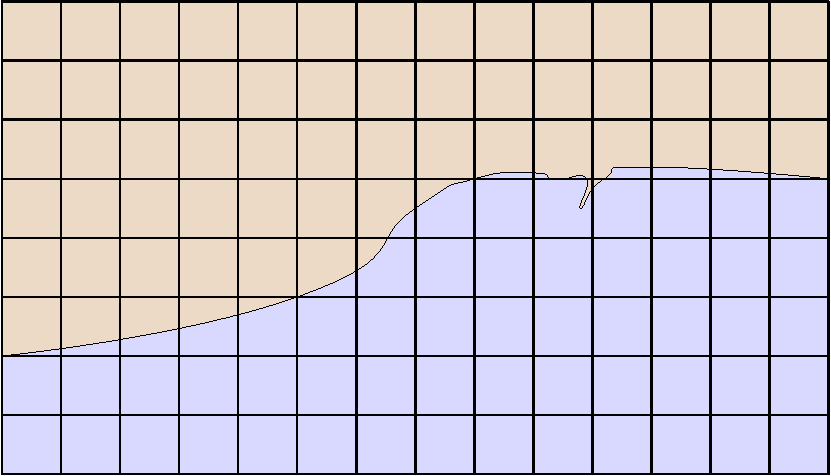
\includegraphics[width=\textwidth]{img/multigrid/grid1.pdf}
    \vspace{1em}
\end{subfigure}
\begin{subfigure}{.8\textwidth}
    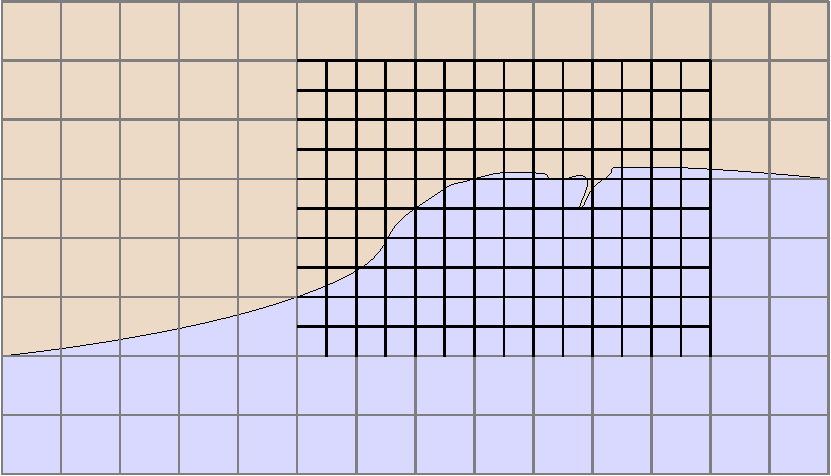
\includegraphics[width=\textwidth]{img/multigrid/grid2.pdf}
    \vspace{1em}
\end{subfigure}
\begin{subfigure}{.8\textwidth}
    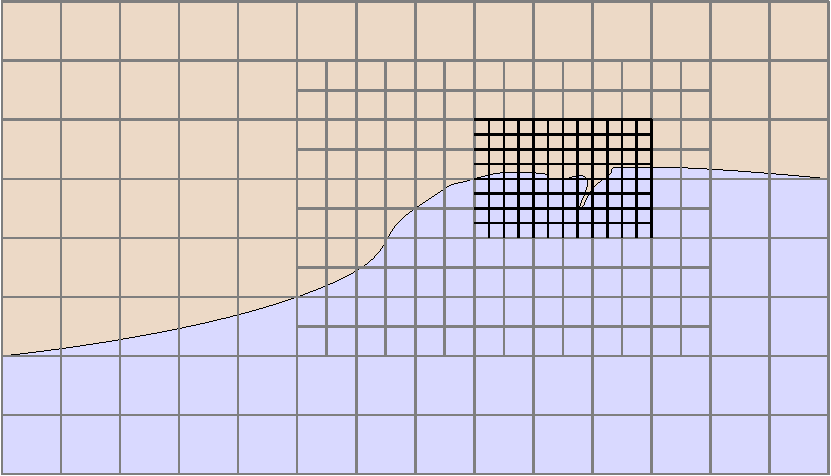
\includegraphics[width=\textwidth]{img/multigrid/grid3.pdf}
    \vspace{1em}
\end{subfigure}
\caption{Different refinement zones for a domain.}
\label{multigrid_refinement}
\end{figure}



\section{Algorithm}


\begin{figure}
    \centering
    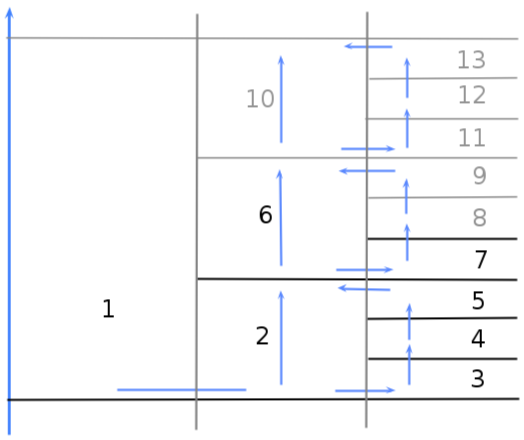
\includegraphics[width=.8\textwidth]{img/multigrid/multigrid_steps.png}
    \caption{Steps for solving a coarse time step with hierarchical refinement.}
    \label{multigrid_steps}
\end{figure}


\section{Data structure}


\section{Refinement criterion}


\section{Examples}



